\documentclass[tikz, border=5pt]{standalone}

\usepackage{tikz}
\usetikzlibrary{arrows.meta, calc}

\begin{document}

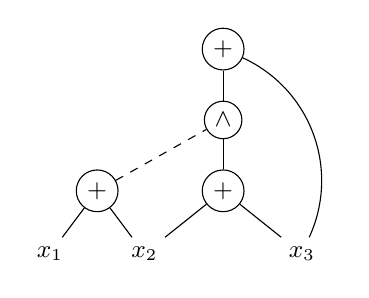
\begin{tikzpicture}[
    gate/.style={circle, draw, inner sep=2pt},
    every node/.style={font=\small}
]

% Inputs
\node (x1) at (0,0) {$x_1$};
\node (x2) at (1.2,0) {$x_2$};
\node (x3) at (3.2,0) {$x_3$};

% XOR(x1,x2)
\node[gate] (xor12) at (0.6,0.8) {$+$};
\draw (x1) -- (xor12);
\draw (x2) -- (xor12);

% XOR(x3)
\node[gate] (xor23) at (2.2,0.8) {$+$};
\draw (x3) -- (xor23);
\draw (x2) -- (xor23);

% AND gate
\node[gate] (and1) at (2.2,1.7) {$\wedge$};
\draw (xor23) -- (and1);

% Top XOR
\node[gate] (xorTop) at (2.2,2.6) {$+$};
\draw (and1) -- (xorTop);

% Curved connection to x3
\draw[bend left=45] (xorTop) to (x3);

% Dashed connection from xor12 to and1
\draw[dashed] (xor12) -- (and1);

\end{tikzpicture}

\end{document}
